\section{Evaluation}

In this section we show that performance of implemented algorithm is in good agreement with theoretical estimations, and that the worst-case time and space complexity can be achieved.
We also present the application of our algorithm to the problem of querying RDF ontologies.

All tests were run on a PC with the following characteristics:
\begin{itemize}
\item OS: Microsoft Windows 10 Pro
\item System Type: x64-based PC
\item CPU: Intel(R) Core(TM) i7-4790 CPU @ 3.60GHz, 3601 Mhz, 4 Core(s), 4 Logical Processor(s)
\item RAM: 32 GB
\end{itemize}


\subsection{Ontology querying}

One of classical graph querying problems is a navigation queries for ontologies, and we apply our algorithm to this problem in order to estimate its practical value.
We used dataset from paper~\cite{CFGonRDF}.
Our algorithm is aimed to process graphs, so RDF files were converted to edge-labeled directed graph.
For each triple $(o,p,s)$ form RDF we added two edges: $(o,p,s)$ and $(s,p^{-1},o)$.

We perform two classical \textit{same-generation queries}~\cite{FndDB}.

\textbf{Query 1} is based on the grammar for retrieving concepts on the same layer (presented in figure~\ref{grammarQ1}).
For this query our algorithm demonstrates up to 1000 times better performance and provides identical results as compared to the presented in~\cite{CFGonRDF} for $Q_1$. 

\textbf{Query 2} is based on the grammar for retrieving concepts on the adjacent layers (presented in figure~\ref{grammarQ2}). 
Note that this query differs from the original query $Q_2$ from article~\cite{CFGonRDF} in the following details.
First of all, we count only triples for nonterminal $S$ because only paths derived from it correspond to paths between concepts on adjacent layers.
Algorithm which is presented in~\cite{CFGonRDF} returns triples for all nonterminals.
Moreover, grammar $\mathcal{G}_2$, which is presented in~\cite{CFGonRDF}, describes paths not only between concepts on adjacent layers.
For example, path ``$\text{\textit{subClassOf} \textit{subClassOf}}^{-1}$'' can be derived in $\mathcal{G}_2$, but it is a path between concepts on the same layer, not adjacent.
We changed the grammar to fit a query to a description provided in paper~\cite{CFGonRDF}. 
Thus results of our query is different from results for $Q_2$ which provided in paper~\cite{CFGonRDF}.

Results of both queries are presented in table~\ref{tbl1}, where \#triples is a number of $(o,p,s)$ triples in RDF file, and \#results is a number of triples of form $(S,v_1,v_2)$.
In our approach result triples can be founded by filtering out all SPPF nonterminal nodes labeled by $(v_1,S,v_2)$.

\begin{figure}[ht]
   \begin{center}
   \[
\begin{array}{rl}
   0: & S \rightarrow \text{\textit{subClassOf}}^{-1} \ S \ \text{\textit{subClassOf}} \\ 
   1: & S \rightarrow \text{\textit{type}}^{-1} \ S \ \text{\textit{type}} \\ 
   2: & S \rightarrow \text{\textit{subClassOf}}^{-1} \ \text{\textit{subClassOf}} \\ 
   3: & S \rightarrow \text{\textit{type}}^{-1} \ \text{\textit{type}} \\ 
\end{array}
\]
   \caption{Grammar for query 1}
   \label{grammarQ1}        
   \end{center}
\end{figure}

\begin{figure}[ht]
   \begin{center}
   \[
\begin{array}{rl}
   0: & S \rightarrow B \ \text{\textit{subClassOf}} \\ 
   1: & B \rightarrow \text{\textit{subClassOf}}^{-1} \ B \ \text{\textit{subClassOf}} \\
   2: & B \rightarrow \text{\textit{subClassOf}}^{-1} \ \text{\textit{subClassOf}} \\ 
\end{array}
\]
   \caption{Grammar for query 2}
   \label{grammarQ2}        
   \end{center}
\end{figure}


\begin{table*}
\centering
\caption{Evaluation results for Query 1 and Query 2}
\label{tbl1}

\begin{tabular}{ | c | c | c | c | c | c |}
\hline
Ontology & \#triples & \multicolumn{2}{|c|}{Query 1} & \multicolumn{2}{|c|}{Query 2} \\
\cline{3-6}
& & time(ms) & \#results & time(ms) & \#results \\
\hline 
\hline
skos        & 252 & 10 & 810 & 1 & 1 \\
generations & 273 & 19 & 2164 & 1 & 0 \\
travel      & 277 & 24 & 2499 & 1 & 63 \\
univ-bench  & 293 & 25 & 2540 & 11 & 81 \\
foaf        & 631 & 39 & 4118 & 2 & 10 \\
people-pets & 640 & 89 & 9472 & 3 & 37 \\
funding     & 1086 & 212 & 17634 & 23 & 1158 \\
atom-primitive & 425 & 255 & 15454 & 66 & 122 \\
biomedical-measure-primitive & 459 & 261 & 15156 & 45 & 2871 \\
pizza       & 1980 & 697 & 56195 & 29 & 1262 \\
wine        & 1839 & 819 & 66572 & 8 & 133 \\
\hline
\end{tabular}

\end{table*}

As a result, we conclude that our algorithm is fast enough to be applicable to some real-world problems.

\subsection{Worst-case Complexity} 

We use two grammars for balanced brackets --- ambiguous grammar $G_0$(fig.~\ref{grammarG0}) and unambiguous grammar $G_2$(fig.~\ref{grammarG2}) --- in order to investigate performance and grammar ambiguity correlation.

\begin{figure}[ht]
   \begin{center}
   \[
\begin{array}{rl}
   0: & S \rightarrow a \ S \ b \ S \\ 
   1: & S \rightarrow \varepsilon
\end{array}
\]
   \caption{Unambiguous grammar $G_2$ for balanced brackets}
   \label{grammarG2}        
   \end{center}
\end{figure}

As input we use complete graphs in which for each terminal symbol there is an edge labeled with it between every two vertices.
Note that we use only terminal symbols for edges labels.  
The task we solve in our experiments is to find all paths from all vertices to all vertices satisfied specified query.
Such designed input looks hard for querying in terms of required resources because there is a correct path between any two vertices and result set is infinite.

For complete graph $M=(V,E,L)$ $$\max\limits_{v \in V}\left(deg^+\left(v\right)\right) = (|V| - 1)*|\Sigma|$$, where $\Sigma$ is terminals of input grammar, hence we should get time complexity $O(|V|^4)$ and space complexity $O(|V|^3)$.

Performance measurement results are presented in figure~\ref{pic:Perf}. 
For time measurement results we have that all two curves can be fit with polynomial function of degree 4 to a high level of confidence with $R^2$. 

%g(x) = m*x**3 + n*x**2 + o*x + p
%fit g(x) 'perf/2' using 1:4 via n,m,o,p

\begin{figure}[ht]
\centering
%\begin{gnuplot}
%set terminal epslatex color size 9cm,8cm
%set yrange [0:]
%set key box top left
%set key width 2
%set key opaque
%set sample 1000
%set xlabel 'Number of vertices in input graph'
%set ylabel 'Time in milliseconds'

%f1(x) = 0.000495989*x**4 + 0.001252184*x**3 + 0.068491746*x**2 - 0.306749160*x
%f2(x) = 0.003368883*x**4 - 0.114919298*x**3 + 3.161793404*x**2 - 22.549491142*x

%plot 'perf/2' using 1:3  pt 6 title '$G_2$',\
%     'perf/2' using 1:4  pt 5 title '$G_0$',\
%     f1(x)  with line lt -1 title '$f_1$',\
%     f2(x)  lc rgb "black" dashtype 2 title '$f_2$'     

% \end{gnuplot}
 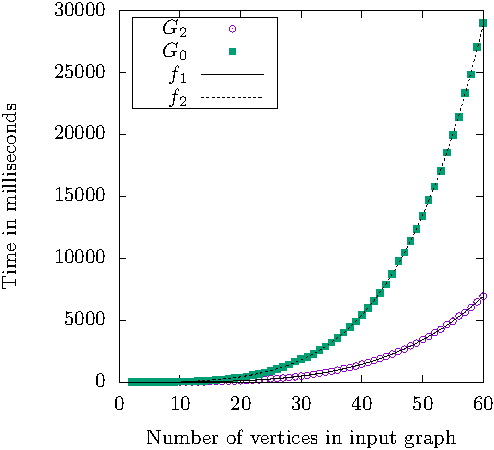
\includegraphics[width=8cm]{dot/grph1.pdf}
\caption{Performance on complete graphs for grammar $G_0$ and $G_2$ \\ 
$f_1(x) = 0.000496*x^4 + 0.001252*x^3 + 0.068492*x^2 - 0.306749*x$; $R^2 = 0.99996$ \\
$f_2(x) = 0.003369*x^4 - 0.114919*x^3 + 3.161793*x^2 - 22.54949*x$; $R^2 = 0.99995$}
\label{pic:Perf}
\end{figure}

Also we present SPPF size in terms of nodes for both $G_0$ and $G_2$ grammars (fig.~\ref{pic:SPPFSize}).
As was expected, all two curves are cubic to a high level of confidence with $R^2 = 1$. 

\begin{figure}[ht]
\centering
%\begin{gnuplot}
%set terminal epslatex color size 9cm,8cm
%set key box top left
%set key width 2
%set key opaque
%set sample 1000
%set xlabel 'Number of vertices in input graph'
%set ylabel 'Number of SPPF nodes'

%f1(x) = 3.000047*x**3 + 3.994579*x**2 + 4.191568*x
%f2(x) = 3.000050*x**3 + 2.994338*x**2 + 4.196472*x


%plot 'perf/2' using 1:6 pt 6 title '$G_2$',\
%     'perf/2' using 1:7 pt 5 title '$G_0$',\
%     f1(x)  with line lt -1 title '$f_1$',\
%     f2(x)  lc rgb "black" dashtype 2 title '$f_2$'     

% \end{gnuplot}
 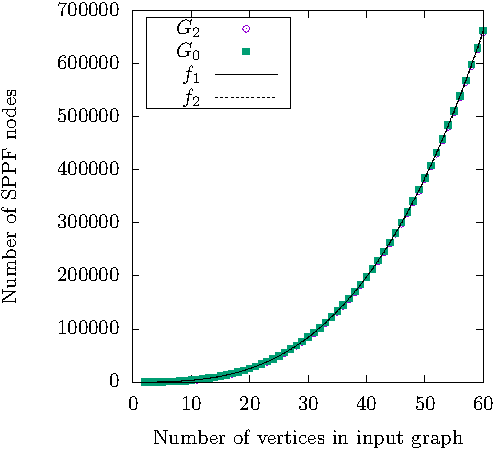
\includegraphics[width=8cm]{dot/grph2.pdf}
\caption{SPPF size on complete graph for grammar $G_0$ and $G_2$ a complete graphs \\
$f_1(x) = 3.000047*x^3 + 3.994579*x^2 + 4.191568*x$; $R^2 = 1$\\
$f_2(x) = 3.000050*x^3 + 2.994338*x^2 + 4.196472*x$; $R^2 = 1$}
\label{pic:SPPFSize}
\end{figure}


%\begin{figure}[h]
%\centering
%\begin{gnuplot}
%set terminal epslatex color size 9cm,8cm
%set key box top left
%set logscale y
%set key width 2
%set key opaque
%set sample 1000
%set xlabel '$x$-label'
%set ylabel '$y$-label
%plot 'perf/3' using 1:2 with lines ls 2 ti '$Unamb$',\
%     'perf/3' using 1:3 with lines ls 3 ti '$amb$'
%
% \end{gnuplot}
%\caption{Performance on C graph for grmmars $G_0$ and $G_2$}
%\label{pic:DoubleCyclesPerf}
%\end{figure}




%To summarise we can say that performance for unambiguos grammars is better then for ambiguos. 

%Full graphs for balanced brackets.

%Full graph for highly unambiguos greammar $G_3$ (figure~\ref{grammarG3}).

%\begin{figure}[h]
%   \begin{center}
%\begin{verbatim}
%   0: s = s s s 
%   1: s = s s
%   2: s = A
%\end{verbatim}
%   \caption{Highly ambiguos grammar $G_3$}
%   \label{grammarG3}        
%   \end{center}
%\end{figure}
